\documentclass[a4paper, table]{article}
% Useful packages, sorted so packages of similar functionality are grouped together. Not all are essential to make the document work, however an effort was made to make this list as minimalistic as possible. Feel free to add your own!

% Essential for making this template work are graphicx, float, tabularx, tabu, tocbibind, titlesec, fancyhdr, xcolor and tikz. 

% Not essential, but you will have to debug the document a little bit when removing them are amsmath, amsthm, amssymb, amsfonts, caption, subcaption, appendix, enumitem, hyperref and cleveref.

% inputenc, lipsum, booktabs, geometry and microtype are not required, but nice to have.

\usepackage[utf8]{inputenc} % Allows the use of some special characters
\usepackage{amsmath, amsthm, amssymb, amsfonts} % Nicer mathematical typesetting
\usepackage{lipsum} % Creates dummy text lorem ipsum to showcase typsetting 

\usepackage{graphicx} % Allows the use of \begin{figure} and \includegraphics
\usepackage{wrapfig}
\usepackage{float} % Useful for specifying the location of a figure ([H] for ex.)
\usepackage{caption} % Adds additional customization for (figure) captions
\usepackage{subcaption} % Needed to create sub-figures
\usepackage{gnuplottex}
\usepackage{tabularx} % Adds additional customization for tables
\usepackage{tabu} % Adds additional customization for tables
\usepackage{booktabs} % For generally nicer looking tables

%\usepackage[ngerman]{babel}
\usepackage[nottoc,numbib]{tocbibind} % Automatically adds bibliography to ToC
\usepackage[margin = 2.5cm]{geometry} % Allows for custom (wider) margins
\usepackage{microtype} % Slightly loosens margin restrictions for nicer spacing  
\usepackage{titlesec} % Used to create custom section and subsection titles
\usepackage{titletoc} % Used to create a custom ToC
\usepackage{appendix} % Any chapter after \appendix is given a letter as index
\usepackage{fancyhdr} % Adds customization for headers and footers
\usepackage[shortlabels]{enumitem} % Adds additional customization for itemize. 
\usepackage{multicol}
\usepackage{multirow}
\usepackage[sorting=none]{biblatex}
 \usepackage{siunitx} % Use SI Units
\usepackage{hyperref} % Allows links and makes references and the ToC clickable
\usepackage[noabbrev, capitalise]{cleveref} % Easier referencing using \cref{<label>} instead of \ref{}

\usepackage{xcolor} % Predefines additional colors and allows user defined colors

\usepackage{tikz} % Useful for drawing images, used for creating the frontpage
\usetikzlibrary{positioning} % Additional library for relative positioning 
\usetikzlibrary{calc} % Additional library for calculating within tikz
\usepackage{listings}

\definecolor{codegreen}{rgb}{0,0.6,0}
\definecolor{codegray}{rgb}{0.5,0.5,0.5}
\definecolor{codepurple}{rgb}{0.58,0,0.82}
\definecolor{backcolour}{rgb}{0.95,0.95,0.92}

\lstdefinestyle{mystyle}{
    backgroundcolor=\color{backcolour},   
    commentstyle=\color{codegreen},
    keywordstyle=\color{magenta},
    numberstyle=\tiny\color{codegray},
    stringstyle=\color{codepurple},
    basicstyle=\ttfamily\footnotesize,
    breakatwhitespace=false,         
    breaklines=true,                 
    captionpos=b,                    
    keepspaces=true,                 
    numbers=left,                    
    numbersep=5pt,                  
    showspaces=false,                
    showstringspaces=false,
    showtabs=false,                  
    tabsize=2
}

\lstset{style=mystyle}

% Defines a command used by tikz to calculate some coordinates for the front-page
\makeatletter
\newcommand{\gettikzxy}[3]{%
  \tikz@scan@one@point\pgfutil@firstofone#1\relax
  \edef#2{\the\pgf@x}%
  \edef#3{\the\pgf@y}%
}
\makeatother

\usepackage[Option]{overpic}

 % Loads in the preamble 
% Give your report a title
\newcommand\reporttitle{Project I}

% Insert course code, name, quartile number and year (or any other subtitle)
\newcommand\reportsubtitle{Applied Data Analysis\\ and Machine Learning
}

% Add your group number (for DBL) or any other text.
%\newcommand\groupnumber{
%\textbf{\LARGE{Involved students:}}
%}

% Insert authors and student numbers here
\newcommand\reportauthors{ 
\rule{0pt}{3ex}  
\LARGE{Johan}\\
\LARGE{Toralf}\\
\LARGE{Peter}\\
\LARGE{Frederik Eichenberger}\\
%\LARGE{3481354} \\
%\LARGE{Sebastian Rentschler} & \LARGE{3471775} \\
}

% Add the name of your tutor (for DBL) or any other text.
\newcommand\grouptutor{
\LARGE{Professor: Morten Hjorth-Jensen}
}

% Date and location (default: current date and Eindhoven)
\newcommand\placeanddate{
Oslo, \today
}

% Define Tue-red (color of the TU/e logo). Can be changed to drastically change the look of the template
\definecolor{Tue-red}{RGB}{199, 25, 24}

% All of the following code can be removed to be left with (close to) default LaTeX behaviour. 

% Sets up hyperlinks in the document to be colored
\hypersetup{
    colorlinks=true,
    linkcolor=Tue-red,
    urlcolor=Tue-red,
    citecolor = Tue-red
    }
\urlstyle{same} % Defines settings for link and reference formatting


% Change bullet style for level 1, 2 and 3 respectively for itemize
\renewcommand{\labelitemi}{\scriptsize\textcolor{Tue-red}{$\blacksquare$}}% level 1
\renewcommand{\labelitemii}{\scriptsize\textcolor{Tue-red}{$\square$}}% level 2
\renewcommand{\labelitemiii}{\textcolor{Tue-red}{$\circ$}}% level 3

% \renewcommand{\labelitemi}{\small\textcolor{Tue-red}{\ding{70}}} % level 1
% \renewcommand{\labelitemii}{\small\textcolor{Tue-red}{\ding{71}}}% level 2
% \renewcommand{\labelitemiii}{\tiny\textcolor{Tue-red}{\ding{71}}}% level 3

% Change bullet style for level 1, 2 and 3 respectively for enumerate
\renewcommand{\labelenumi}{\textbf{\textcolor{Tue-red}{\arabic*.}}}% level 1
\renewcommand{\labelenumii}{\textbf{\textcolor{Tue-red}{[\alph*]}}}% level 2
\renewcommand{\labelenumiii}{\textbf{\textcolor{Tue-red}{\roman*.}}}% level 3

% Have reference labels be linked to section (section 3 will have fig. 3.1 etc.)
\counterwithin{equation}{section} % For equations
\counterwithin{figure}{section} % For figures
\counterwithin{table}{section} % For tables

% Creates a beautiful header/footer
\pagestyle{fancy}
%\lhead{\includegraphics[height = 8pt]{Figures/0. General/Logo Bild.jpg}}
\rhead{\reporttitle}
\renewcommand{\footrulewidth}{0.4pt}
\cfoot{Page \thepage}

% Formats section, subsection and subsubsection titles respectively 
\titleformat{\section}{\sffamily\color{Tue-red}\Large\bfseries}{\thesection\enskip\color{gray}\textbar\enskip}{0cm}{} % Formats section titles

\titleformat{\subsection}{\sffamily\color{Tue-red}\large\bfseries}{\thesubsection\enskip\color{gray}\textbar\enskip}{0cm}{} % Formats subsection titles

\titleformat{\subsubsection}{\sffamily\color{Tue-red}\bfseries}{\thesubsubsection\enskip\color{gray}\textbar\enskip}{0cm}{} % Formats subsubsection titles

% Formats captions
\DeclareCaptionFont{Tue-red}{\color{Tue-red}}
\captionsetup{labelfont={Tue-red,bf}}

 % Changes font to mlmodern
\usepackage{mlmodern}

% Removes indent when starting a new paragraph
\setlength\parindent{0pt}

% Limits the ToC to sections and subsections (no subsubsec.)
\setcounter{tocdepth}{2}
 % Loads in user defined
\addbibresource{General/References.bib}

\begin{document}

% Inserts the front page
\begin{titlepage}

\centering

\begin{tikzpicture}

%\node[opacity=0.3,inner sep=0pt,remember picture,overlay] at (4.5,-0.5){\includegraphics[width= 0.8 \textwidth]{Figures/0. General/Logo Bild.jpg}};

\node[inner sep=0pt] (logo) at (0,0)
   {
\includegraphics[width=.5\textwidth]{Figures/0. General/02_uio_full_logo_eng_pos.jpg}};
    
\node[text width = 0.5\textwidth, right = of logo](title){\sffamily\huge\reporttitle};

\node[text width = 0.5\textwidth, yshift = 0.75cm, below = of title](subtitle){\sffamily\Large \reportsubtitle};

\gettikzxy{(subtitle.south)}{\sffamily\subtitlex}{\subtitley}
\gettikzxy{(title.north)}{\titlex}{\titley}
\draw[line width=1mm, Tue-red]($(logo.east)!0.5!(title.west)$) +(0,\subtitley) -- +(0,\titley);

\end{tikzpicture}
\vspace{3cm}

\sffamily\groupnumber

\begin{table}[H]
\centering
\sffamily
\large
\begin{tabu} to 0.8\linewidth {c}
\textbf{\LARGE{Involved students}} \\
%\textbf{\LARGE{Student ID}}\\
\hline

\sffamily\reportauthors

\end{tabu}

\end{table}

\sffamily \grouptutor


\\ \ \\ \ \\
\begin{flushright}
\small{Picture by \href{https://flickr.com/photos/dalbera/4840429336/}{Annie Dalbéra}. \href{https://creativecommons.org/licenses/by/2.0/deed.de}{CC BY 2.0}}
\end{flushright}
\tikz[remember picture,overlay]\node[anchor=south,inner sep=0pt] at (current page.south) {
\includegraphics[width=\paperwidth, height=13cm]{Figures/0. General/Oslo image.jpg}};

\mbox{}
\vfill
\sffamily \Large \textcolor{white}{\placeanddate } \\
\end{titlepage}









\newpage

% Generates a ToC without page number
{\hypersetup{linkcolor=black} % Keeps the ToC black even with non-black linkcolor
\tableofcontents\thispagestyle{empty}}
\newpage


\section{Abstract} \label{section:Abstract}
In this project linear regressions methods will be used to create a model fitting to geographic topological data of the area of Kathmandu. Therefore, ordinary least square method and Ridge and Lasso methods will be applied, using data sampled from resampling techniques such as bootstrap method or cross-validation. 
\section{Introduction} \label{section:Exercise 2}
Regression methods are applied in various different fields, ranging from cancer prediction methods \cite{SHAIKH202240}, financial risk assessment \cite{BROBY2022145} and also in climate and emission research it has found its applications \cite{ZhouYi}. In this project we are trying to apply machine learning methods onto geographic topological data, to find function representing the terrain of a certain area. First the methods of Ordinary least squares (OLS), Ridge and Lasso regression will be presented and tested on a three dimensional Franke-function with a small noise. The methods will be evaluated depending depending on their complexity using the mean squared error. Furthermore, resampling techniques such as cross-validation and a bootstrap method will be used to create more available datapoints. \\
In the second step OLS will be used to fit geographic data from Kathmandu.  \\


\section{Franke-function}\label{section:Franke-function}
To develope an understanding of different linear regression methods, the Franke-function will serve as an example. The Franke function is defined as:
\begin{equation}
    \begin{split}
        %\begin{align*}
f(x,y) &= \frac{3}{4}\exp{\left(-\frac{(9x-2)^2}{4} - \frac{(9y-2)^2}{4}\right)}+\frac{3}{4}\exp{\left(-\frac{(9x+1)^2}{49}- \frac{(9y+1)}{10}\right)} \\
&+\frac{1}{2}\exp{\left(-\frac{(9x-7)^2}{4} - \frac{(9y-3)^2}{4}\right)} -\frac{1}{5}\exp{\left(-(9x-4)^2 - (9y-7)^2\right) }.
        %\end{align*}
    \end{split}
\end{equation}
For our purpose we will reduce the function to the interval $x,~y \in [0,~1]$ and add a small stochastic noise $\varepsilon \sim \mathcal{N}(0,~0.1)$ on top. The Frankie is displayed in figure...

% Insert figure


\subsection{Ordinary least squares}
In the first step Ordinary least squares (OLS) will be used to find a function fitting the Franke-function. The mean squared error (MSE) is given by
\begin{equation}
    MSE(\boldsymbol{y},\tilde{\boldsymbol{y}}) = \frac{1}{n}
\sum_{i=0}^{n-1}(y_i-\tilde{y}_i)^2,
\end{equation}
which will be used as a cost function. Different complexity models will be analyzed, calculating the MSE and $R^2$-value depending on the polynomial degree, which are displayed in figure \ref{fig:MSE-R2}. 

% Update figure with other colors, also pdf format
\begin{figure}
    \centering
    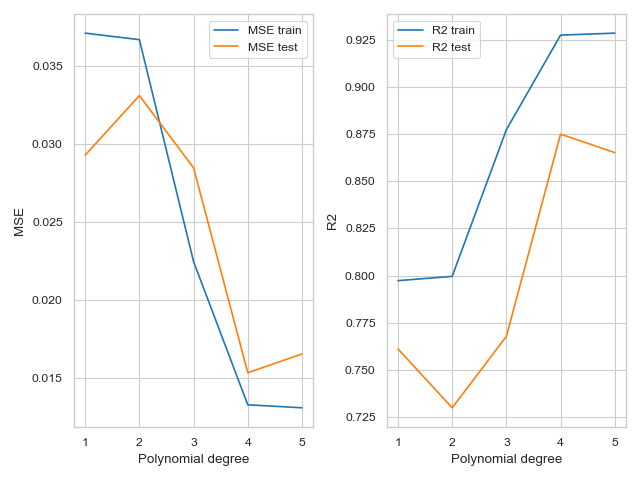
\includegraphics[width=0.9\textwidth]{Figures/1. Franke-function/franke_OLS_mse_r2.png}
    \caption{MSE and $R^2$-value of Ordinary least square fitting the Franke-function for training and test data. }
    \label{fig:MSE-R2}
\end{figure}


The data is split using 70\% as training and 30\% as test data. And the MSE is evaluated for a polynomial polynomial degree up to 5. 





\subsection{Part (d)} \label{section:Exercise 1}
%\setlength{\columnseprule}{1pt}
%\def\columnseprulecolor{\color{Tue-red}} % Creates a red line seperating the colums

%\begin{multicols}{2} % To use a two column page
%\end{multicols}
\begin{equation}
    y = f(x) + \varepsilon, ~~\text{with} ~\varepsilon \sim \mathcal{N}(0, \sigma^2)
\end{equation}
For the Expectation value it is obtained
\begin{equation}
\mathbb{E}[y_i] = \mathbb{E}[f(x) + \varepsilon_i] = 
\underbrace{\mathbb{E}[f(x_i)]}_{\sum_j x_{ij} \beta_j} + 
\underbrace{\mathbb{E}[\varepsilon_i]}_{=0} = 
\sum _j x_{ij}\beta_j = \textbf{X}_{j*} \boldsymbol\beta
\end{equation}
The variance is given by
\begin{equation}
\begin{split}
    \text{Var}(y_i) = \text{Var}[f(x_i) + \varepsilon_i] & = \text{Var}[f(x_i)] +\underbrace{\text{Var}[\varepsilon_i]}_{\sigma^2} + 2\cdot \underbrace{\text{Cov}[f(x_i), \varepsilon_i]}_{=0} \\
   & = \mathbb{E}[f(x_i)^2] - \mathbb{E}[f(x_i)]^2 + \sigma^2 \\
   & = f(x_i)^2 - f(x_i)^2 + \sigma^2 \\
   & = \sigma ^2
    \end{split}
\end{equation}
The expectation value of $\hat\beta$ is given by
\begin{equation}
    \mathbb{E}[\boldsymbol{\hat\beta}] = \mathbb{E}[(\boldsymbol{X}^T\boldsymbol{X})^{-1}\boldsymbol{X}^T\boldsymbol{y}] = (\boldsymbol{X}^T\boldsymbol{X})^{-1} \boldsymbol{X}^T\cdot \underbrace{\mathbb{E}[\boldsymbol{y}]}_{\boldsymbol{X}\boldsymbol\beta} = (\boldsymbol{X}^T\boldsymbol{X})^{-1}\boldsymbol{X}^T\boldsymbol{X}\boldsymbol\beta = \boldsymbol\beta 
\end{equation}
With a variance of 
\begin{equation}
    \begin{split}
    \text{Var}[\boldsymbol{\hat\beta}] = & \mathbb{E}\left\{(\boldsymbol{\hat\beta}-\mathbb{E}[\boldsymbol{\hat\beta}])(\boldsymbol{\hat\beta}-\mathbb{E}[\boldsymbol{\hat\beta}])^T\right\} 
    \\ = & \mathbb{E}\left\{
    \left((\boldsymbol{X}^T\boldsymbol{X})^{-1}\boldsymbol{X}^T\boldsymbol{y} - \boldsymbol\beta\right)
    \left((\boldsymbol{X}^T\boldsymbol{X})^{-1}\boldsymbol{X}^T\boldsymbol{y} - \boldsymbol\beta\right)^T\right\} 
    \\ = & \mathbb{E}\left\{
    (\boldsymbol{X}^T\boldsymbol{X})^{-1}\boldsymbol{X}^T\boldsymbol{y}
    ((\boldsymbol{X}^T\boldsymbol{X})^{-1}\boldsymbol{X}^T\boldsymbol{y})^T
    + \boldsymbol\beta\boldsymbol\beta^T \\
    & - \boldsymbol\beta\boldsymbol{y}^T\boldsymbol{X}(\boldsymbol{X}^T\boldsymbol{X})^{-1}
    -(\boldsymbol{X}^T\boldsymbol{X})^{-1}\boldsymbol{X}^T\boldsymbol{y}\boldsymbol\beta^T\right\}
    \\ = &
    \mathbb{E}\left\{\boldsymbol{X}^T\boldsymbol{X})^{-1} \boldsymbol{X}^T \boldsymbol{y} \boldsymbol{y}^T \boldsymbol{X} (\boldsymbol{X}^T\boldsymbol{X})^{-1} \right\} + \boldsymbol{\beta \beta}^T 
    \\ & - \boldsymbol{\beta}\boldsymbol{\beta}^T \boldsymbol{X}^T\boldsymbol{X} (\boldsymbol{X}^T\boldsymbol{X})^{-1}
    - (\boldsymbol{X}^T\boldsymbol{X})^{-1} \boldsymbol{X}^T\boldsymbol{X}\boldsymbol{\beta}\boldsymbol{\beta}^T\\
    = & \mathbb{E}\left\{\boldsymbol{X}^T\boldsymbol{X})^{-1} \boldsymbol{X}^T \boldsymbol{y} \boldsymbol{y}^T \boldsymbol{X} (\boldsymbol{X}^T\boldsymbol{X})^{-1} \right\}
    - \boldsymbol{\beta \beta}^T \\
    \end{split}
\end{equation}
where 
\begin{equation}
    \mathbb{E}[\boldsymbol{yy}^T] = \boldsymbol{X\beta\beta}^T\boldsymbol{X}
\end{equation}
This yields for the variance
\begin{equation}
    \begin{split}
    \text{Var}[\boldsymbol\hat\beta] = & (\boldsymbol{X}^T\boldsymbol{X})^{-1}(\boldsymbol{X}^T\boldsymbol{X}) \boldsymbol{\beta\beta}^T
    + (\boldsymbol{X}^T\boldsymbol{X})^{-1}\boldsymbol{X}^T\sigma^2\boldsymbol{X} (\boldsymbol{X}^T\boldsymbol{X})^{-1} - \boldsymbol{\beta\beta}^T\\
    = & \sigma^2 (\boldsymbol{X}^T\boldsymbol{X})^{-1}
    \end{split}
\end{equation}

\subsection{Part (e)}

\begin{equation}
    \begin{split}
    \mathbb{E}\left[ (\boldsymbol{y} - \boldsymbol{\tilde{y}})^2\right] = 
    \mathbb{E}\left[ (f(x) + \varepsilon - \boldsymbol{\tilde{y}})^2\right]
    = & \mathbb{E}\left[f(x)^2 + \varepsilon^2 - \boldsymbol{\tilde{y}}^2
    + 2 f(x) \varepsilon - 2f(x) \boldsymbol{\tilde{y}} - 2 \varepsilon \boldsymbol{\tilde{y}}\right]\\
    = & \mathbb{E}\left[ f(x)^2 + \boldsymbol{\tilde{y}}^2  - 2 f(x)\boldsymbol{\tilde{y}}\right] + \sigma^2\\
    \end{split}
\end{equation}
Introducing a 'smart 0', given through the expression $\mathbb{E}[\boldsymbol{\tilde{y}}]- \mathbb{E}[\boldsymbol{\tilde{y}}]= 0$,
we can separate the terms above towards
\begin{equation}
    \begin{split}
        \mathbb{E}\left[ (\boldsymbol{y} - \boldsymbol{\tilde{y}})^2\right] =
        \underbrace{\mathbb{E}[(f(x)-\mathbb{E}[\boldsymbol{\tilde{y}})^2]}_{(\text{Bias}(\boldsymbol{\tilde{y}}))^2}
        + 
        \underbrace{\mathbb{E}[(\boldsymbol{\tilde{y}}}_{\text{Var}(\boldsymbol{\tilde{y}})} - \mathbb{E}[\boldsymbol{\tilde{y}})^2] + 
        \mathbb{E}[(f(x) - \mathbb{E}[\boldsymbol{\tilde{y}}])(\underbrace{\mathbb{E}[\boldsymbol{\tilde{y}}] - \boldsymbol{\tilde{y}})}_{=0}] + \sigma^2
    \end{split}
\end{equation}
Thus we finally obtain
\begin{equation}
    \mathbb{E}\left[ (\boldsymbol{y} - \boldsymbol{\tilde{y}})^2\right] =
    \left[\text{Bias}(\boldsymbol{\tilde{y}})\right]^2 + \text{Var}(\boldsymbol{\tilde{y}}) + \sigma^2
\end{equation}
\input{Chapters/04. Geographic data}
\input{Chapters/05. Conclusion}

% Generates a list of symbols table
%\input{Chapters/0. List of symbols}


%\pagenumbering{arabic}




% Creates references using the Biblatex 
%\bibliographystyle{unsrt} % Different style of displaying references
%\bibliography{General/References.bib}
\newpage
\printbibliography
\newpage

\appendix % Any section after this command will have a letter as an index

% Adds an appendix entry


\end{document}
